\documentclass[thesis]{plai}

\usepackage{tabularx}

\usepackage{lipsum}
\usepackage{booktabs}
\usepackage{graphicx}
\usepackage{tabularx}
\usepackage{svg}
\graphicspath{{images/}}
\usepackage{rotating}
\usepackage{float}
\usepackage{fancyhdr}
\setlength{\headheight}{13.6pt}
\addtolength{\topmargin}{-1.6pt}
\usepackage{microtype}
\usepackage{color}
\definecolor{light-gray}{gray}{0.80}
\usepackage{placeins}
\usepackage[ruled,vlined,linesnumbered]{algorithm2e}
\SetKw{Continue}{continue}
\newcommand\mycommfont[1]{\footnotesize\ttfamily\textcolor{blue}{#1}}
\SetCommentSty{mycommfont}
\usepackage{tikz}
\usetikzlibrary{backgrounds,
  shapes.geometric,
  arrows,
  decorations,
  decorations.pathreplacing,
  fit,
  positioning,
  shapes.multipart,
  calc,
  trees,
  graphs,
  quotes,
  matrix }
\usepackage{adjustbox}
\tikzstyle{class} = [rectangle, draw=black, fill=blue!20, text width=6em, align=center, rounded corners, minimum height=2em]
\tikzstyle{block} = [draw, rectangle, text width=2cm, text centered, minimum height=1.2cm, node distance=3cm,fill=white]
\tikzstyle{method} = [text width=6em, align=left]
\usepackage{multirow}
\newcommand{\specialcell}[2][c]{%
  \begin{tabular}[#1]{@{}l@{}}#2\end{tabular}}

\usepackage{amsthm}

\theoremstyle{definition}
\newtheorem{definition}{Definition}

\usepackage{enumitem}
\usepackage{glossaries}
% Compiling with `pdflatex` will generate the glossary!
\newglossaryentry{plai}
{
  name = PLAI,
  description = {The coolest research group in the entire universe},
}
\newglossaryentry{dse}
{
  name = DSE,
  description = {Dynamic Symbolic Execution},
}
\newglossaryentry{api}
{
  name = API,
  description = {Application Programming Interface},
}
\newglossaryentry{http}
{
  name = HTTP,
  description = {Hyper Text Transfer Protocol},
}
\newglossaryentry{crud}
{
  name = CRUD,
  description = {Persistent Database operations: Create, Read, Update, Delete},
}
\newglossaryentry{html}
{
  name = HTML,
  description = {Hypertext Markup Language},
}
\newglossaryentry{vi}
{
  name = PLAI,
  description = {The coolest research group in the entire universe},
}
\newglossaryentry{vii}
{
  name = PLAI,
  description = {The coolest research group in the entire universe},
}
\makeglossaries

% ---------------------------------------------- %
\pretitle{}
\posttitle{}
\title{
    \begin{center}
        \bfseries\LARGE
        Security testing of web applications with dynamic symbolic execution in expoSE
    \end{center}
}
\preauthor{}
\postauthor{}
\author{
    \begin{center}
        \large
        Moritz Böhm
    \end{center}
}
\predate{}
\postdate{}
\date{\relax}

% ---------------------------------------------- %
\begin{document}


\begin{center}
    \uppercase{Ludwig-Maximilians-Universität München}
\end{center}

\begin{center}
    \uppercase{Chair of Programming Languages and Artificial Intelligence}
\end{center}

\vspace*{10mm}

\begin{center}
    \includegraphics[height=40mm]{sigillum.png}
\end{center}

\vspace*{10mm}

{\let\newpage\relax\maketitle}

\thispagestyle{empty}

\begin{center}
    \begin{large}
        \begin{Large}
            Master's Thesis \\
        \end{Large}
        in course type Computer Science\\
    \end{large}
\end{center}

\vspace{1cm}

\begin{center}
    \begin{large}
        Supervisor: Prof. Dr. Johannes Kinder\\
    \end{large}
\end{center}

\begin{center}
    \begin{large}
        Advisor: Advisor's name\\
    \end{large}
\end{center}


\begin{center}
    \begin{large}
        Submission Date: \today{}\\
    \end{large}
\end{center}

\vspace{1,5cm}

\cleardoublepage{}

\thispagestyle{empty}

\vspace*{20mm}
\noindent

\makeatletter

\begin{center}
    {\textbf{Disclaimer}}
\end{center}

\begin{flushleft}
    {I confirm that this Master's Thesis is my own work and I have documented all sources and material used.}

    \makeatother

    \vspace{15mm}
    \noindent

    Munich, \today{}

    Moritz Böhm
\end{flushleft}

\cleardoublepage{}


\thispagestyle{empty}

\vspace*{20mm}

\begin{center}
    \makeatletter

    {\textbf{Acknowledgments}}

    \makeatother
\end{center}

\begin{flushleft}
    I would like to express my heartfelt gratitude to everyone who has supported me throughout the journey of this thesis.
    
    Special thanks to Professor Kinder, for introducing me to this truly fascinating topic of \textit{dynamic symbolic execution} and for enabling me to write this thesis, while providing his continuous support and help over the course of this project.
\capstartfalse

\end{flushleft}

\vspace{10mm}

\cleardoublepage{}


\chapter*{Abstract}

As web applications grow in complexity and prevalence, ensuring their security and reliability has become increasingly important.
This thesis explores the use of Dynamic Symbolic Execution (DSE) through the ExpoSE framework to automate web application testing.
Specifically, we aim to evaluate whether ExpoSE can effectively identify bugs and security vulnerabilities, with a particular focus on Cross-Site Scripting (XSS) attacks.

Our approach involves merging the client and server into a single entity, enabling DSE to generate paths based not only on the client’s state but also on server internals.
The research includes the design and implementation of an Express.js model to facilitate the testing of complex web applications.
Through systematic evaluations, we demonstrate ExpoSE’s ability to generate inputs that cover application routes and decision paths, thereby revealing both functional issues and security weaknesses.
Our findings show that ExpoSE was able to generate unique test cases and find potential vulnerabilities related to input handling and validation.


\newpage
\tableofcontents
\newpage

\setcounter{page}{1}
\pagestyle{fancy}
\fancyhf{}
\fancyhead[R]{\thepage}
\renewcommand{\headrulewidth}{0pt}
\raggedbottom
% ---------------------------------------------- %
\chapter{Introduction}
\label{chapter:introduction}
\pagenumbering{arabic}
\setcounter{page}{1}
\section{Motivation}
\label{sec:motivation}

Whenever we write code, testing is an essential process that cannot be overlooked. Ideally, testing occurs concurrently with development; failing to do so can lead to unpleasant surprises later on. Bill Gates once remarked, 
\begin{quote}

    “… we have as many testers as we have developers. And testers spend all their time testing, and developers spend half their time testing. We're more of a testing, a quality software organization than we're a software organization.” — Bill Gates in an interview for InformationWeek \cite{bill_q_2002} 
\end{quote}

This statement underscores the critical role of testing in software development—an endeavour that can be even more important than writing the code itself.


The severity of bugs and vulnerabilities varies significantly based on the application's nature and context. For instance, an offline program has different security considerations than an Internet of Things (IoT) application, such as a smart thermostat, or a web application handling sensitive data globally. Each of these programs can harbour security issues, necessitating extensive testing to identify potential flaws. As software becomes increasingly complex, catching all bugs becomes increasingly challenging. 


Consequently, automating this time-consuming testing process is a highly sought-after goal, leading to numerous approaches aimed at achieving it.
Dynamic Symbolic Execution (DSE) is one approach that has gained traction for automating test coverage and uncovering software bugs and vulnerabilities. While DSE can be traced back to the early 1970s, with foundational work by \citet{boyer_selectformal_1975} and \citet{king_new_1975}, it has recently experienced a resurgence. Numerous frameworks for DSE have been developed, each with its advantages and limitations. Among them, ExpoSE, as described in \citet{loring_expose_2017}, stands out for its strength in string manipulation and reasoning critical features when testing web applications, where data is predominantly transmitted in text-based formats and requires string operations such as checking whether a string matches a certain pattern or splitting it into multiple parts.



\newpage

\section{Research questions}
\label{sec:research-questions}

This thesis aims to apply DSE using the ExpoSE framework to test web applications and to answer the following research questions:

\begin{itemize}
    \item RQ1: Is it possible to reliably end-to-end fuzz test a web application using Dynamic Symbolic Execution in ExpoSE?
    \item RQ2: Can it be used to reliably locate security issues?
\end{itemize}

We tested two web applications and our results indicated that it is indeed possible to end-to-end fuzz test a web application with DSE in ExpoSE, which allowed us to proceed to answer RQ2.
In this thesis, we paid special attention to vulnerabilities known as Cross-Site Scripting (XSS), which is a prevalent issue in web applications. XSS attacks can allow malicious actors to execute scripts in the context of a user's browser, potentially leading to unauthorized actions, data theft, and other security concerns. Given ExpoSE's robust support for string operations, we believed it is well-suited to identify such string-based attacks, which turned out to be true, answering RQ2 successfully.

\section{Structure}
\label{sec:thesis-structure}
This thesis is structured as follows. First, we will explain the terminology and the theories this thesis builds on. 
Following this, we proceed to provide a description of ExpoSE and its technologies, along with an overview of its usage.
Next, we present the necessary changes for ExpoSE to function and outline our approach to the problem addressed in this thesis. This chapter also offers a minimal answer to RQ1.
Expanding on this foundation, we will delve into the application of a JavaScript framework, detailing the model created for it and explaining its necessity. 
An evaluation of our approach follows,  where we test the model within a web application and provide an answer to our research question, reflecting on whether we have met our goals.
We then will offer a review of related work in the field of symbolic execution, highlighting significant research and methodologies relevant to our study. 
Finally, we will conclude the thesis, presenting an overview of what we achieved and learned.

% ---------------------------------------------- %
\chapter{Background}
\label{chapter:background}
In order to address the research inquiries posed in~\autoref{sec:research-questions}, it is imperative to first comprehend the subjects and their fundamentals. 

We start by defining the topic areas touched upon by this thesis~(\autoref{sec:defs}), then explain the technologies used within the tool ExpoSE ~(\autoref{sec:defs}), and finally explain the limitations imposed by the engine itself~(\autoref{sec:limits}). 

\section{Definitions}
\label{sec:defs}
To provide an overview of all the topics that will be addressed, we will begin by defining the key components of this thesis and explaining the basics to build upon in the later chapters. 
\subsection{Web Applications}
\label{sec:webapp}
A \textit{web application} has been defined as “a software application, executed by a web server, which responds to dynamic web page requests over HTTP” by the Web Application Security Consortium (WASC) ~\cite{noauthor_web_2012}. 
In simpler terms, a web application is software that runs on a server and users access it through a web browser (like Chrome or Firefox) over the internet.

Typically, the resources and scripts of web applications — such as images, text, or functionalities — are requested by the client, which is the user's computer or device, using a web browser or similar tools. This interaction follows a set of rules known as the API (Application Programming Interface), which specifies what requests can be made and how the server should respond.
The~\autoref{fig:simplified-web-app} illustrates the basic communication process between the client (the user's device), the server (where the application runs), and external services (such as another server).


Most web applications also use a database, which is a structured way of storing data, to keep information consistently available and reliable. For the purposes of this discussion, we assume that the web application has a monolithic architecture. This means that it operates as a single cohesive program on a physical computer, as opposed to being divided into separate parts that run on different cloud services (like AWS, or Amazon Web Services, which offers online computing power without needing dedicated hardware)~\cite{noauthor_serverless_nodate}.
Additionally, we assume the server follows REST (Representational State Transfer) principles, which are guidelines for how web services should operate to enable smooth communication as described by \citet{roy_t_fielding_rest_2008}. 
The web server processes requests that adhere to the HTTP (Hypertext Transfer Protocol) standard, which is the foundational protocol used for transmitting data on the web (ref. ~\autoref{tab:rest_http_methods}).
This adherence ensures that the server and client can operate independently, meaning they can be developed and updated separately without affecting each other\cite{fielding_http_2022}.

\begin{figure}[h]
    \centering
    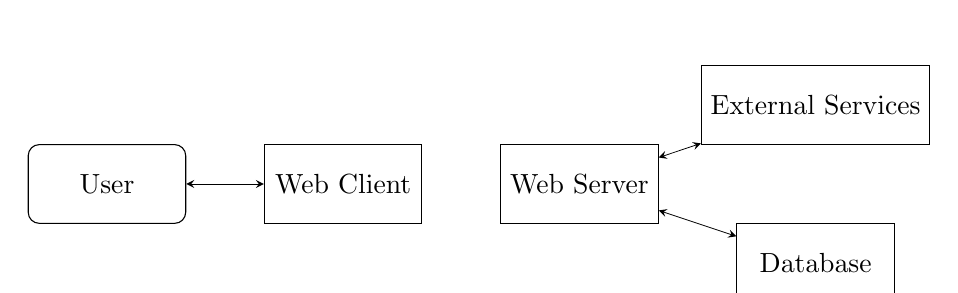
\begin{tikzpicture}[node distance=3cm]
    % Define styles for nodes and arrows
    \tikzstyle{user} = [rectangle, rounded corners, minimum width=2cm, minimum height=1cm, text centered, draw=black]
    \tikzstyle{browser} = [rectangle, minimum width=2cm, minimum height=1cm, text centered, draw=black]
    \tikzstyle{server} = [rectangle, minimum width=2cm, minimum height=1cm, text centered, draw=black]
    \tikzstyle{database} = [rectangle, minimum width=2cm, minimum height=1cm, text centered, draw=black]
    \tikzstyle{external} = [rectangle, minimum width=2cm, minimum height=1cm, text centered, draw=black]
    % Use arrows with both directions
    \tikzstyle{arrow} = [thick, <->, >=stealth]
% Arrow style for double lines

    \tikzset{doubleArrow/.style={thick, <->, >=stealth,
        line width=0.1mm, line cap=round, draw=black
    }}
    % Nodes
    \node (user) [user] {User};
    \node (browser) [browser, right of=user] {Web Client};
    \node (server) [server, right of=browser] {Web Server};
    \node (database) [database, right of=server, yshift=-1cm] {Database};
    \node (external) [external, right of=server, yshift=1cm] {External Services};
    % Arrows (connections)
    \draw  [doubleArrow](user) -- (browser);
    \draw  [doubleArrow](server) -- (database);
    \draw [doubleArrow] (server) -- (external);
    \end{tikzpicture}
    \caption{Structure of a simplified Web Application}
    \label{fig:simplified-web-app}

\end{figure}

\begin{table}[htb]
    \centering
    \begin{tabular}{@{}lll@{}}
        \toprule
        \textbf{HTTP Method} & \textbf{Purpose}                         & \textbf{Idempotent} \\ \midrule
        GET                   & Retrieve a resource                     & Yes                 \\
        POST                  & Create a new resource                   & No                  \\
        PUT                   & Update or create a resource             & Yes                 \\
        PATCH                 & Partially update a resource             & Yes (mostly)        \\
        HEAD                  & Retrieve headers of a ressource         & Yes                 \\
        OPTIONS               & Return available HTTP methods           & Yes                 \\
        DELETE                & Remove a resource                       & Yes                 \\ \bottomrule
    \end{tabular}
    \caption{Summary of REST HTTP Methods and their idempotence \cite[chapter 9]{fielding_http_2022}}
    \label{tab:rest_http_methods}
\end{table}
\FloatBarrier
\subsection{Testing}
\label{sec:testing}

The next part we want to focus on is testing a web application. First we define what "testing" means, then look into the methodology of "fuzzing" as a technique used to test. We limit this to the following two testing paradigms: White Box Fuzzing (\autoref{sec:white-box}) and Black Box Fuzzing (\autoref{sec:black-box}).

\subsubsection{Testing}
At its essence, \textit{Testing} constitutes the systematic process of validating and verifying the functionality of a program. A sensible analogy for the concepts of validation and verification was articulated by B. W. Boehm \citet{b_w_boehm_verifying_1984}. 

\begin{itemize}[label={}]
    \item \textit{Verification}: "Am I building the product right?" 
    \item \textit{Validation}: "Am I building the right product?"
\end{itemize}
Depending on the nature of the testing methodology employed, different levels of assessment can be achieved. A unit test, which is designed to evaluate a single component or function—hence the term "unit"—primarily provides insights into the correctness of that individual function. In contrast, an end-to-end test, while potentially less precise in verifying the functionality of individual components, serves to validate the overall functionality of the entire system. 

Given that a program can accommodate a vast array of potential inputs, it may be impractical to manually identify all possible variations. Therefore, we can utilize a technique known as "fuzzing."

\subsubsection{Fuzzing}
\label{sec:fuzzing}
\textit{Fuzzing} is an automated process that involves the generation of input data to identify potential program errors, commonly referred to as "bugs," which may arise from unhandled edge cases. These edge cases can include scenarios such as incompatible data types, excessively large entities, or the presence of unexpected characters.
Fuzzing can be done in different ways and in the following we will describe the two most commonly used types: "white-box fuzzing" and "black-box fuzzing".


\vspace{0.5cm}
\begin{tabular*}{\textwidth}{@{}c|c@{}}
    
\begin{minipage}{\dimexpr0.5\textwidth-2\tabcolsep}
\centering
    % Left Diagram - White Box Fuzzing
    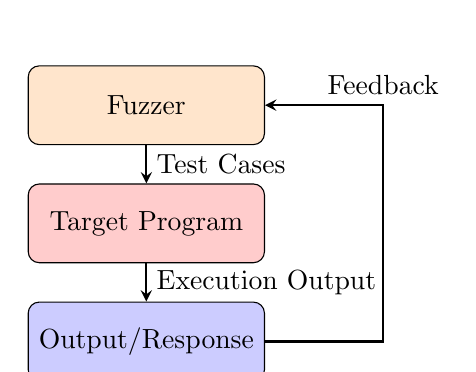
\begin{tikzpicture}[node distance=1.5cm]
                % Define styles for nodes and arrows
        \tikzstyle{box} = [rectangle, rounded corners, minimum width=3cm, minimum height=1cm, text centered, draw=black, fill=blue!20]
        \tikzstyle{fuzzer} = [rectangle, rounded corners, minimum width=3cm, minimum height=1cm, text centered, draw=black, fill=orange!20]
        \tikzstyle{target} = [rectangle, rounded corners, minimum width=3cm, minimum height=1cm, text centered, draw=black, fill=red!20]
        \tikzstyle{arrow} = [thick,->, >=stealth]
        \tikzstyle{title} = [rectangle, rounded corners, minimum width=5cm, text centered, draw=none, fill=none, font=\large\bfseries] 
    
        \node (fuzzer) [fuzzer] {Fuzzer};
        \node (target) [target, below of = fuzzer] {Target Program};
        \node (output) [box, below of = target] {Output/Response};

        % Arrows
        \draw  [arrow](fuzzer) -- (target) node[midway, right] {Test Cases};
        \draw [arrow] (target) -- (output) node[midway,right] {Execution Output};
        \draw [arrow] (output.east) --+(1.5,0) |- (fuzzer.east) node[midway, above] {Feedback};
    \end{tikzpicture}

\end{minipage}
&
\begin{minipage}{\dimexpr0.5\textwidth-2\tabcolsep}
\centering

    % Left Diagram - White Box Fuzzing
    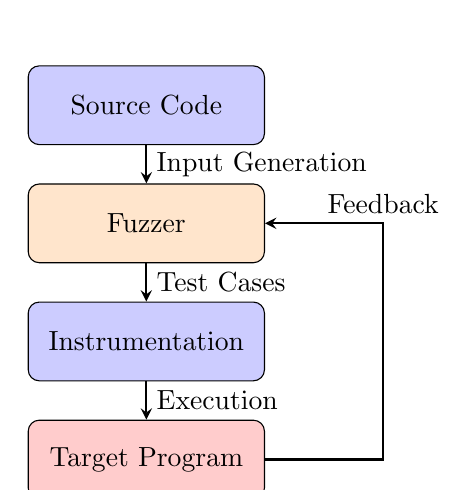
\begin{tikzpicture}[node distance=1.5cm]

        \tikzstyle{box} = [rectangle, rounded corners, minimum width=3cm, minimum height=1cm, text centered, draw=black, fill=blue!20]
        \tikzstyle{fuzzer} = [rectangle, rounded corners, minimum width=3cm, minimum height=1cm, text centered, draw=black, fill=orange!20]
        \tikzstyle{target} = [rectangle, rounded corners, minimum width=3cm, minimum height=1cm, text centered, draw=black, fill=red!20]
        \tikzstyle{arrow} = [thick,->, >=stealth]
        \tikzstyle{title} = [rectangle, rounded corners, minimum width=5cm, text centered, draw=none, fill=none, font=\large\bfseries]
        \node (source) [box] {Source Code};
        \node (fuzzer) [fuzzer, below of = source] {Fuzzer};
        \node (instr) [box, below of = fuzzer] {Instrumentation};
        \node (target) [target, below of = instr] {Target Program};

        % Arrows
        \draw  [arrow](source) -- (fuzzer) node[midway, right] {Input Generation};
        \draw  [arrow](fuzzer) -- (instr) node[midway, right] {Test Cases};
        \draw  [arrow](instr) -- (target) node[midway, right] {Execution};
        \draw  [arrow](target.east) -- +(1.5,0) |- (fuzzer.east) node[midway, above] {Feedback};

    \end{tikzpicture}
    
\end{minipage}

\\

\begin{minipage}[t]{\dimexpr0.5\textwidth-1\tabcolsep}
\captionof{figure}{Simplified black-box fuzzing process}
    \label{fig:black-box-testing}

\end{minipage}
&
\begin{minipage}[t]{\dimexpr0.5\textwidth-1 \tabcolsep}
\captionof{figure}{Simplified white-box fuzzing process}
\label{fig:white-box-testing}

\end{minipage}

\end{tabular*}

\subsubsection{Black Box Fuzzing}
\label{sec:black-box}
\textit{Black box fuzzing} (ref. \autoref{fig:black-box-testing}) is a software testing method that evaluates an application’s security and robustness by feeding it random or semi-random inputs without any knowledge of its internal workings—such as source code, data structures, or algorithms. This approach simulates an external attacker's perspective, enabling testers to discover vulnerabilities that might be exploited by malicious users in a real-world scenario.

The key characteristic of black-box fuzzing is its lack of insight into the internal design and logic of the software being tested. Instead, the focus is on the inputs and outputs of the application. Testers generate a wide variety of input data, often using automated tools or scripts, to gauge how the application responds. This can include testing edge cases, invalid inputs, or unexpected data formats to determine how robust the application is against improper use.

One of the main advantages of black-box fuzzing is its simplicity and ease of use. Since testers do not need to understand the details of the application’s code, they can quickly implement fuzzing without extensive knowledge of the underlying logic. This makes black-box fuzzing an attractive option for assessing third-party software or legacy applications where source code is not available.

Black-box fuzzing can be effective in identifying common security vulnerabilities, such as buffer overflows, input validation errors, and unexpected crashes. By observing how the application behaves with various inputs, testers can pinpoint areas of insecurity, allowing developers to focus their remedial efforts on the most critical issues.

Though black-box fuzzing offers valuable insights into application security, it does have some limitations. Specifically, the randomness of the generated inputs might not exercise all potential execution paths, leaving some vulnerabilities undiscovered. Furthermore, without knowledge of the internal code structure, it can be challenging to prioritize which vulnerabilities are more critical based on potential impact.

In conclusion, black-box fuzzing is an essential technique within the realm of software security testing. By simulating external attacks and evaluating the application solely based on its inputs and outputs, this method helps identify significant vulnerabilities that can compromise the application’s integrity. While it may lack the depth of white-box approaches, black-box fuzzing remains a crucial tool in the arsenal of security professionals, enabling them to enhance the overall security posture of applications in a comprehensive manner. \cite{godefroid_random_2007}

\subsubsection{White Box Fuzzing}
\label{sec:white-box}
\textit{White box fuzzing} (ref. \autoref{fig:white-box-testing}) is an advanced software testing technique that seeks to identify vulnerabilities and bugs within applications by utilizing an in-depth understanding of their internal structures and logic. Unlike traditional black-box testing methods, where testers approach the software without any knowledge of its internal workings, white-box fuzzing leverages access to the source code, algorithms, and data flows, allowing for a more targeted and effective analysis.

One of the primary benefits of white-box fuzzing is its ability to generate test inputs based on the actual paths and branches present in the code. By analyzing the control flow and data structures inherent to the application, white-box fuzzers can create specific input cases that exercise various execution paths. This targeted approach increases the likelihood of uncovering potential weaknesses, particularly in areas of the code that may be prone to errors or security vulnerabilities.

Additionally, white-box fuzzing often incorporates dynamic analysis. During the fuzzing process, the application is executed in a controlled environment, and its behavior is monitored in real-time. This provides valuable feedback on how the program reacts to the generated inputs, enabling the identification of unhandled cases that may lead to crashes, incorrect outputs, or security flaws.

Another critical feature of white-box fuzzing is coverage measurement. By measuring code coverage, testers can ensure that their input generation strategies are effective in exercising different paths within the software. This helps identify areas of the code that have not been adequately tested, enabling a more comprehensive examination of the program's reliability and security.

The primary objective of white-box fuzzing is to detect issues such as buffer overflows, null pointer dereferences, and other runtime errors that could compromise an application’s stability or allow for security breaches. By identifying these vulnerabilities early in the development process, organizations can address them proactively, ultimately enhancing the overall quality and security of their software.

In summary, white-box fuzzing is a powerful and efficient technique for software testing, combining knowledge of internal application structures with automated input generation and dynamic monitoring. This method significantly contributes to improving the robustness and security of software applications by exposing vulnerabilities that may be overlooked in traditional testing approaches.\cite{godefroid_random_2007}




\subsection{Dynamic Symbolic Execution}
\label{sec:dse}
\textit{Dynamic symbolic execution} (DSE) is a technique similar to white-box fuzzing, as it requires access to the source code. However, instead of requiring an actual input, it assumes that the variables are "symbolic," meaning that they do not possess a tangible value during execution of the program. Instead, it tracks the conditions encountered during runtime, generating constraints based on the symbolic variables. This facilitates a comprehensive examination of multiple program pathways, thereby aiding in the identification of anomalies that may result in unforeseen behaviour or security vulnerabilities.

After exploring a particular execution path, DSE employs constraint solvers to analyse the constraints collected during execution. These solvers determine concrete inputs that can satisfy the path constraints, allowing the generation of specific test cases to trigger particular code paths during subsequent executions.

By integrating DSE into white-box fuzzing, testers can automatically generate test cases that reliably expose bugs or vulnerabilities, such as buffer overflows or access violations. This allows for a more exhaustive testing process that can reveal flaws that traditional fuzzing techniques might overlook.

The synergy between DSE and white-box fuzzing promotes automated test generation and increases the coverage of tested paths, ultimately improving the software's reliability and security. It provides developers with concrete inputs that reproduce identified vulnerabilities, facilitating easier debugging and remediation.

In summary, dynamic symbolic execution significantly enhances the capabilities of white-box fuzzing by providing a structured, thorough, and automated approach to analyze program behavior. It helps identify and confirm vulnerabilities through the intelligent exploration of execution paths, making it a powerful tool in software testing and security analysis.

Let us proceed through the process of generating the path conditions (abbrv. PC) by employing the ensuing code snippet (\autoref{fig:code-snippet}). 
\begin{figure}[ht]
    \begin{lstlisting}[language=JavaScript, gobble=4, escapechar=@]
    function g(x) {
        if (x < 0){
            x=-x;
        }
        else {
            if (x === 0){
                x=1;
            }
            x = x + 1;
        }
        if (!(x >0)){
            x =-1;
        }
    }
    \end{lstlisting}
    \caption{A simple program}
    \label{fig:code-snippet}
\end{figure}


\subsection{SMT Solver}
\label{sec:smtsolver}

A \textit{satisfiability modulo theories }(SMT) Solver, is used to solve mathematical and logical problems. 

\section{Tech Stack}
\label{sec:tech}
In this section, we will delve into the inner workings of the expoSE framework, what tools it uses and their function within.


\subsection{Jalangi}
\label{sec:jalangi}

Jalangi2 is used in order to instrument the javascript code that is to be analyzed. 
\begin{figure}[ht]
    \begin{lstlisting}[language=JavaScript, gobble=4]
    J$.iids = {"8":[9,7,9,14],"9":[2,10,2,17],"10":[6,6,6,11]...,"nBranches":6}
    [...]
    x = J$.N(257, 'x', x, 4);
    if (J$.X1(345, J$.C(16, J$.B(10, '<', J$.R(89, 'x', x, 0), J$.T(97, 0, 22, false), 0)))) {
        J$.X1(121, x = J$.W(113, 'x', J$.U(18, '-', J$.R(105, 'x', x, 0)), x, 0));
    } else {
        [...]
    }
    [...]
    }

    \end{lstlisting}
    \caption{A simple program snippet, instrumented by JALANGI2}
    \label{fig:code-snippet}
\end{figure}
 
\subsection{Z3 SMT Solver}
\label{sec:z3}


ExpoSE uses the Z3 SMT Solver for solving the found path conditions of the analysed program. Developed by Microsoft, it has constant progress and improvements to its capabilities. 

\subsection{Z3Javascript}
\label{sec:z3js}

Z3Javascript is an extension for Z3 to generate JavaScript bindings to be used in ExpoSE.


\subsection{expoSE}
\label{sec:expose}
So, what exactly is this ominous "ExpoSE" we keep on talking about? 
In short, it is a DSE Framework for JavaScript, which allows almost any (explanation why almost see \autoref{sec:limits}), to be tested for reachability and bugs.



% ---------------------------------------------- %
\chapter{Implementation}
\label{chapter:implementation}


This chapter provides an overview of the project in \autoref{sec:overview}, outlines the necessary modifications to the existing project to execute expoSE on the execution platform in\autoref{sec:fwd-z3}, and presents the discovered system-imposed limitations in \autoref{sec:limits}. It then presents the initial idea in \autoref{sec:init-test-plain}. Some of them were contingent upon the platform on which the program was executed. In this case, an Apple MacBook Pro with an M1 Pro chip. 

\section{Overview}
\label{sec:overview}


ExpoSE functions as depicted in \autoref{fig:expose-struc} starting from a component referred to as the distributor to orchestrate the process of symbolic execution. The distributor facilitates the transmission of inputs to the executor, which, as its designation implies, executes the program under test utilizing these inputs. The execution of the program produces a trace, which is subsequently returned to the executor. From this trace, the path condition corresponding to the input is communicated to the SMT Solver. The SMT Solver solves the constraints and then transmits the resulting model back to the executor, enabling the executor to extrapolate alternative inputs. These alternative inputs are subsequently relayed to the distributor, thereby initiating the entire process again. In scenarios where multiple alternative inputs are generated, these inputs are executed concurrently.

For our case, the program under test is not just one script, but consists of both the server and the client, but also of the express model, the request model and the response model. 



\begin{figure}
  \centering
\includegraphics{exposeArchitectureDiagram.pdf}
 \caption{Express model structure, as depicted in \cite{loring_practical_2021}, modified to depict the web application}
     \label{fig:expose-struc}
\end{figure}


\FloatBarrier
\section{Forwarding Changes of Z3}
\label{sec:fwd-z3}
This section provides a short overview of the changes made to two of the four main parts that make up ExpoSE. Both were relatively simple in nature, but they were required to fix a z3 specific internal error, that kept occurring and caused the execution to fail.

\subsection{Changes to z3}
\label{sec:changes-z3}
As the forked repository of z3 made for expoSE was almost 5 years old, and we occasionally noticed a null pointer exception in the c++ code, we decided to pull the changes from the original repository into the fork, almost 5000 commits, in the hopes of that the null pointer exception has been fixed meanwhile. 
The forwarding went smoothly, with two exceptions. Z3 now includes the type “Char Pointer”, which had to be added to the JavaScript portion (and the Python part, as JavaScript basically copies the bindings from Python) of the binding creation.

The second exception was, that the z3 API now provided a few more callbacks, which, however, required parameters that were not implemented for JavaScript. We have chosen to eliminate these components from our fork over implementing them, as they were not utilized in expoSE and resulted in the failure of the binding generation.

\subsection{Changes to z3JavaScript}
\label{sec:changes-z3js}
With the update to z3 itself, we also had to update the z3JavaScript project, as this defined the types for the JavaScript bindings. It turned out to be a simple issue of adding two new object types (a ParserContextObj and a SimplifierObj) of the type voidp, which is a pointer to the type void.


\section{System-imposed limitations}
\label{sec:limits}
In this section, we will explain the limitations imposed on the application, what it means and how we can circumvent  some of them, while others are a hard  limit.
\subsection{JavaScript Version}
\label{sec:jsversion}
We will start off with the hardest limitation of the application, and that is the fact, that we have to stay in syntax constructs offered by the JavaScript version known as ES6 (or ECMA 2015).

This is a significant limitation, as it implies that we are unable to utilize an essential feature of contemporary JavaScript, specifically \textit{async} and \textit{await}. These two keywords refer to the asynchronous pattern that modern JavaScript employs. Without these, we will not be able to build a modern application, which is a major limitation for a server that might have to wait for resources to load or for a computation-intensive process. For these processes, we now have to rely on callbacks. 



\subsection{HTTP Protocol}
\label{sec:httpprot}
Another limit imposed on us was the communication between client and server, as typically, this would happen using HTTP. However, this would mean that we would lose the symbolic state of the program, as the transfer would occur as a byte stream with all data first transformed into a string representation. 
A string, however, cannot be of symbolic type. \\
This means, we had two options:\\
Option A would require us to model the complete HTTP object, with all its bells and whistles, and then include the symbolic state of the program, all while complying with the HTTP standard. This way, we could also test HTTP, and whether the JavaScript implementation works as intended.

Option B is to bypass the transmission of data entirely, by injecting the server into the client, or vice versa, depending on the server structure (more on that later). This would mean that we would have the full symbolic state of the execution, the data would not need to be transformed, and could simply be handed over to the request and response processing on server- and client-side.


We deemed the modelling of the HTTP object out of scope. Therefore, we worked under the assumption, that HTTP works as intended and went for option B, as that meant, we could focus on the actual web application, and could test it in isolation.


\subsection{Symbolic Objects}
\label{sec:sym-obj}
While the other limits are specific to our use case, this issue is an universal one, as pointers can cause a problem on most symbolic execution engines as described by \citet{cha_unleashing_2012}, \citet{coppa_rethinking_2017} and \citet{elkarablieh_precise_2009}, just to name a few. The biggest culprits in javascript are symbolic objects, as they themselves have a pointer to a memory address, which holds the references for both parts of the key value pair, with the contents of these parts being pointers to another memory address. This poses a problem for discerning what the keys and the values should be, where they are stored and how they are accessed. A purely symbolic object therefore is unfeasible and should be avoided. However, a concrete object may hold symbolic values.

\subsection{External Packages}
\label{sec:externalpack}
Our last hard limit was that, even though it was possible to import and use external packages, the DSE engine would assume that any imported package was part of the code. Although technically true, it meant it would be instrumented and create execution branches. This led to a massive explosion in branches, and while it could be used to find bugs and errors in these external packages aswell, it did not offer any use for locating issues in the part of the web application we wanted to test. 
Hence, we opted out of using any external package for now.

\subsection{Dependency Issues}
\label{sec:dep-issues}
While this was not a limit per se, it proved to be an issue with executing the tool chain of expoSE in the first place. When the codebase was created in 2017, almost all personal use computers were made on an x86 platform. While ARM was already widespread in mobile devices, few personal computers were running on an ARM instruction set\footnote{We assume this to be the case, as even the \href{https://www.arm.com/-/media/global/company/investors/Arm\%20Strategic\%20Review\%20-\%202017.pdf?revision=8473a535-6f7e-4ce5-85fe-0eb6f1f75487&la=en}{investor report} in 2017 does not mention them}. Therefore, little to no effort was spent on supporting it. 
With the release of the M1 processor by Apple, this was no longer the case.
This meant that the ARM instruction set went from being rarely supported to a widely spread one.
When we started working on this thesis, we noticed the lack of support. The project required Node version 14, and the package ffi-napi\footnote{https://www.npmjs.com/package/ffi-napi}, that provided the ability to create C bindings, which were used in z3, required Node 16 or higher.
Upgrading the node version initially, would in turn create an error in ffi-napi for the ARM-based M processors~\footnote{As reported in issue https://github.com/node-ffi-napi/node-ffi-napi/issues/248}.\\
While working on this project, the issue got resolved.



\section{Initial Test Plain JS Application}
\label{sec:init-test-plain}
After addressing all the fundamental issues, we began by creating a small server in plain JavaScript to explore whether it is possible to generate requests, process them, and return the correct response for the request. For example, a GET request with the URL '/test' is handled by a GET route registered as '/test', and not incorrectly by the POST route. 

\subsection{Idea}

The objective was to construct a plain JavaScript server by utilizing the http package's method “createServer” and subsequently eliminating all components that depend on http, thus skipping the actual server-client connection.
We had two goals for this: 
\begin{itemize}
    \item  We created a server that had both static and variable routes, notably one route that consisted only of a regular expression, to test whether all routes could be found by the symbolic variable for the path alone.
    \item  We also implemented a short test for injecting code into the response, by asserting that the client cannot send any script tag \lstinline{<script><\script>} in the request data, while asserting that it has to be a valid email. Which in turn meant, expoSE has to try to violate the assertion, by creating inputs, that contain a script tag and are no valid emails. 
\end{itemize}
For the client side we created a bare-bones client, that was generating the symbolic request, and passed it over to the server by calling the onRequest method of the server, which gets called whenever a request is sent, thereby bypassing HTTP. 

\subsection{Evaluation}
This, albeit small test application, showed us, by fulfilling both of our expected outcomes, that it indeed is possible to test a server with expoSE. Finding all the request routes within the server was straightforward, with a minor drawback: the regular expression route was not functional in a switch-case construct due to its use as a literal and not as a regular expression to match a string. 
The second objective was only moderately successful, as, despite demonstrating theoretically that the generation of a string containing a script tag works, it often exceeded the timeout limit, with a few exceptions in a test of 50 runs, where a matching string was immediately generated.

Despite this, we deemed the initial test application a success, as it strongly suggested that it is possible to test a server, explore all possibly routes and locate issues in the validation, data processing and usage of this data. Hence, we moved on from plain JavaScript to the usage of a framework, in our case, Express.js.


% ---------------------------------------------- %
\chapter{Express Model}
\label{chapter:express}
This chapter introduces a model implementation of the javascript server framework Express.js to to allow for testing using expoSE. 

\section{General Structure}

This section provides an explanation of the general structure of the model and the internal logic of the routing, request handling, with a particular focus on the parametrized routing logic. 

\subsection{Routing} 

Being the most crucial component of any server, routing must be designed accordingly to enable all the features ExpressJS provides, while removing all the ones intended for handling a genuine HTTP request. This means that the model mimics how Express builds its internal routing stack, handles any incoming request, and manipulates the response.  


\subsection{Request Handling}
\subsection{Parametrized Routing}
It is noteworthy that the extraction of parameters sent as route variables must remain symbolic, for instance, when the route is defined as seen in \autoref{fig:param-route}, the request path might look like \lstinline[language=JavaScript, gobble=4]{var path = S.symbol("path", "/user/1");//}. This id then gets extracted from the path, resulting in an Object containing the key (the path variable name) and values (the request path value) seen in \autoref{fig:param-extracted}

\begin{figure}[ht]
    \begin{lstlisting}[language=JavaScript, gobble=4]
    router.get('/user/:id', callback) 
    \end{lstlisting}
    \caption{Parameterized route}
    \label{fig:param-route}
\end{figure}




\begin{figure}[ht]
    \begin{lstlisting}[language=JavaScript, gobble=4]
    const params =  {
        keys: [ 'id' ],
        values: [
        ConcolicValue {
          concrete: '1',
          symbolic: [Expr],
          _arrayType: undefined
    }
  ]
}
    \end{lstlisting}
    \caption{Parameters extracted from the request path}
    \label{fig:param-extracted}
\end{figure}




\section{Peculiarities}
Specific features of the implementation due to the peculiarities of dynamic symbolic execution
%\subsection{Implicit vs Explicit conditionals}
%\subsubsection{re.match}

\section{Usage}
\subsection{Necessary Modifications}
\subsection{Testing}\'?

% ---------------------------------------------- %
\chapter{Application}
\label{chapter:application}
This chapter presents how to use the express model and how to test a web application. 

\section{Necessary Modifications} 
\label{sec:nec-mods}

Since the model is located in expoSE right now, all it requires is a slight modification to the imports and how express is called.
This means, the import requires the relative path, and cannot be imported via the node package manager (NPM). 
The usage is also slightly different, as the express model instance needs to be initiated after importing, while express itself is initiated when it is imported. 
Other than that, it can be used just like express.js, as the basic methods are implemented.





\section{Testing} 
\label{sec:app-testing}
To carry out the end-to-end testing of a web application, we require a client that has the following properties:\\ 
First, it must utilize the S\$ library, which serves as the interface to ExpoSE, as explained in \autoref{sec:expose}. 
Subsequently, all variables within the request should be substituted with symbolic inputs. 
In instances where the server expects a complex data structure in the body of the request,
it is advisable to send an object encapsulating all fields that the server can process across all routes.
This recommendation stems from the challenges associated with symbolic objects, as discussed in \autoref{sec:sym-obj}. 
This approach allows for the generalization of a single test without necessitating multiple executions to cover all required fields,
as any fields not utilized by the specific route are ignored. 
A client such as  \autoref{lst:client-example} could be used to generate the requests.

\begin{lstlisting}[language=JavaScript, float, caption={[Example Client]An Example Client for symbolic requests}, label={lst:client-example}]
const S$ = require("S$");
const { Request } = require("../request");
const { Response } = require("../response");
import HttpMethods from "../express_model/http_methods.enum";


generateRequest (){
    const req  = new Request(
        S$.symbol("path", "/"),
        HttpMethods[S$.symbol("method", 0)],
        {
            "field": S$.symbol("data", "")
        }
    )
    return req;
}
\end{lstlisting}
As explained in \autoref{sec:init-test-plain}, we use our mock implementation for the request and response objects. In the \lstinline{generateRequest} function, we build the symbolic request, which has at least 2 parameters, a URL, and an HTTP method. For the URL parameter, we create a symbolic variable \lstinline{path}, with the seed input \lstinline{"/"}, eliminating all variable types but string. 
We then pass an array containing all http methods, accessing the element via the symbolic index variable \lstinline{method}, with a starting seed like before, to indicate it being an integer.
Additionally, we create an object containing a symbolic field, which corresponds to an expected field in the server. As previously mentioned, we do not recommend using a symbolic object.


Testing a web application using the model is a straightforward process.
By injecting the client into the server code and invoking the \textsc{listen}
function  that typically converts an input into an HTTP request, \lstinline{let response = server.listen('8080,callback, << SYMBOLIC } \par\noindent\lstinline{CLIENT REQUEST >> );}, it becomes feasible to generate inputs that test all routes, incorporating various parameters and bodies.


Once the client is either modified or created to produce a symbolic request, 
a singular execution of ExpoSE should suffice to generate diverse requests that effectively cover all possible paths of a request and trigger all potential unique responses, as long as it is a distinct and reachable path.  

Of course, there also exists the option to unit test the server functions without any need for a client and the express model. However, this does not leverage the power of symbolic execution, as it only generates inputs for a function, instead of the whole system, requiring, albeit few, manual generation of tests for each function.


% ---------------------------------------------- %

\chapter{Evaluation}
\label{chapter:evaluation}
In this chapter, we will describe our methodology and approach in regard to testing the underlying model (as explained in \autoref{chapter:express}) and evaluating our results, finally answering the research questions posed in \autoref{sec:research-questions}. 
The developed model provides the ability to test an express web application fully and thorough, with two points of caution, discussed in \autoref{sec:peculiarities}.

\section{Methodology} 
We had two goals for this endeavour: Answering whether ExpoSE can be used to reliably end-to-end fuzz test a web application, and whether it can be used to locate security issues.

As testing a web application for security issues depends on ExpoSE being able to reliably end-to-end fuzz test a web application, we had to achieve this goal first. After all, should it not be possible to do so, locating security issues is merely dependent on luck, which effectively leaves it unsuitable for its intended purpose. 

To evaluate whether we achieved the first goal with our express model, we use the existing test framework of ExpoSE. With the slight modification that, instead of running the various test files, we used it to run our test server multiple times in parallel, trying to verify that ExpoSE generates inputs that consistently find all available routes and branches within.


For the purpose of testing our model and the capabilities of ExpoSE regarding its applicability to web applications, we first developed one web application ourselves (project A), and to verify its compatibility with real-world projects, we took an existing GitHub project\footnote{https://github.com/rwieruch/node-express-server-rest-api}, that worked within the limits of ExpoSE stated in \autoref{sec:limits} (project B). This means, it was written with the syntax available in ES6 and could easily be stripped of external packages. In this case, the only external package was the CORS package, used for cross-origin resource sharing. It also did not rely on any external database. Hence, it was the perfect example project for our needs. Besides removing the package, we modified the project for use with ExpoSE as presented in \autoref{sec:nec-mods}. This is our project B.
We do not force ExpoSE to generate an input by giving assertions about the form and content of the data, to keep the discovery of paths to the framework. This is to ensure that the normal program flow happens, thus representing a normal execution. 

Project A has a total of six routes, \lstinline[language=JavaScript]+GET, POST, PUT, PATCH, DELETE+, with \lstinline[language=JavaScript]+PATCH+ and one \lstinline[language=JavaScript]+GET+ 
being parameterized routes. It uses three middleware layers for pre-processing a request, and one layer for post-processing the response. Behind each route exists a controller, a service, and a database mock-up, to simulate depth. The parametrized routes are the only which have corresponding functions in the mock database, as they cover generating inputs based on the entries and the conditions for retrieving and updating these. The client used for this application is bare-bones. All it does is generate a request and receive a response, comparing the input with the output. The client is also the only place which holds a reference to the symbolic execution interface 
\lstinline[language=JavaScript]{S$}. 

Project B has a total of eight routes, with 4 of them using path parameters.
It also uses one middleware layer for pre-processing a request, and one layer for post-processing the response. The routing, however, is split into three different routers, which tests our express model's capabilities to work with multiple routers. In this project, the routes hold the executing functions directly. It has no database, but uses objects to store the data. Similar to project A, the client is also bare-bones with the only purpose to generate requests, and check the output. 

The requests for both projects encompass a symbolic number, accessing an array holding strings with HTTP methods, a symbolic string for the URL and an object with concrete field namespaces holding symbolic values.


Due to its heavy memory size requirements, and the fact that it can make use of multicore processing, we ran ExpoSE for our tests on a machine with an AMD EPYC 9654 with 96 cores and 1536 GB of Memory in courtesy of the PLAI Chair.


\section{Results}
\label{sec:results}

To validate our underlaying model, we created project A in such a manner that all available methods were covered: adding middleware, adding routes, and adding router objects.

We split our tests into two categories: general testing, and specific tests for testing whether it is possible to discover security related issues.



\subsection{General Test Result Project A}
With this project, we aimed at building a test that covers all parts of the express model.

On a singular run basis, we analysed the process in depth.
Our analysis indicated that ExpoSE can only reason and generate inputs that match a route, but cannot generate path conditions for the route based on our mock database (an array containing objects). It covered the cases, whether an entry exists or not solely by chance. The requests \lstinline[language=JavaScript]{GET /getWithId/0} and \lstinline[language=JavaScript]{GET /getWithId/2222} are generated inputs, with the former retrieving the user in the object and the latter returning an error response. This also was true for the PATCH requests, where the input \lstinline[language=JavaScript]{PATCH /patch/0} 
triggered the update of an already existing entry, and \lstinline[language=JavaScript]{PATCH /patch/22} returned the expected an error response.



To test the reliability of the model, we executed 100 iterations, yielding  the results as presented in \autoref{tab:results-project-one}. 
In these 100 iterations, ExpoSE generated a total of 1931 inputs, representing unique paths within the iteration, with the minium of found paths being 4 and a maximum of 25. On average, it generated 19.3 inputs, with  a median of 20.5. Almost all iterations generated errors, with an average of 2.66 per iteration, but when replaying ExpoSE with these inputs, we found that none of them were actual errors, as the execution ran without errors.
It did, however, consistently run into the aforementioned timeout of ExpoSE, which is 30 minutes, or 1800 seconds, for a test case.

The most interesting number of the results is that only 7 inputs were generated that matched the basic \lstinline[language=JavaScript]{GET /get} 
route, whereas \lstinline[language=JavaScript]{GET /getWithId/:id} were discovered by almost all runs. 
If we look at the run with the most paths, we can observe the inputs and their count of paths per methods in \autoref{lst:project-a-inputs}.
\begin{lstlisting}[language=JavaScript, float, label={lst:project-a-inputs}, caption={[Generated Inputs for Project A]The inputs generated for project A, listed by the HTTP method, grouped by the router.}]
"GET":      "/":1, 
            "":1, 
            "/get":1, 
            "ABCDEFGHJKL ":1,
            "/getWithId/222":1,
            "/getWithId/0":1
            
"POST"      :"":1,
            "?":1,
            "/post":2
            
"PUT":      "":1, 
            "?":1, 
            "/put":1
            
"PATCH":    "":1, 
            "?":1, 
            "/patch/2":1
            
"DELETE":   "":1, 
            "?":1, 
            "/delete":1
            
"A":        "":1,
            "?":1
"?":        "":1,
            "?":1
"":         "":1,
            "?":1
\end{lstlisting}
This run almost completely explored the entire web application, except for updating an existing entry with 
\lstinline[language=JavaScript]+/patch/0+
, for which ExpoSE cannot create a path condition without an explicit check. 
On the other hand, we did observe runs that almost completely failed to generate inputs that cover routes, as the only route it did find was the base route \lstinline+"/"+.\\
\lstinline[language=JavaScript]+"GET":{"/":1},"POST":{"":1},"PUT":{"?":1},"?":{"?":1}+ were the only inputs generated. 
We could not reproduce this issue, but we assume it happened due to an unhandled error of Z3, as neither ExpoSE nor Jalangi created an error. 

\begin{table}[t]
    \centering
    \begin{tabular*}{\linewidth}{c|c|c}
        \begin{tabular}[t]{lc}
    	\toprule
        Route  & Count\\
        \midrule
        \lstinline+GET /get+    & 7     \\
    	  \lstinline+POST /post+ & 96   \\
    	\lstinline+PUT /put+    & 63    \\
        \lstinline+PATCH /patch/:id+   & 41  \\
        \lstinline+DELETE /delete+ & 96  \\
        \lstinline+GET /getWithId/:id+  & 51  \\                    
    	\bottomrule
        \end{tabular}
& 
       \begin{tabular}[t]{ccc}
       	\toprule
                & Paths & Runtime \\
            \midrule

        Min     &4      & 7s     \\
        Max     &   25      & 3611s       \\
        Median  &  20.5  &   1808s        \\   
        Total   &    1931     &   \\
        \bottomrule
        \end{tabular} 
&     

        \begin{tabular}[t]{cc}
        \toprule
    	\multicolumn{2}{c}{Errors} \\
            \midrule

            False & 266 \\
            True  & 0 \\
            Total &  266  \\
    	    \bottomrule
            \end{tabular}
\\
        \end{tabular*}
	\caption[General results of project A]{ Results of 100 ExpoSE runs on project A.
	The first major column is listing the routes with their HTTP method and URL, with a count across all iterations. The second major column containing the columns paths and runtime lists the minimum, the maximum, and the median of paths generated and time taken respectively. The last major column errors depict the number of errors generated by ExpoSE, of which we
	verified whether they were “true” errors or false positives. }
	\label{tab:results-project-one}
\end{table}



\FloatBarrier
\subsection{General Test Result Project B}

Since we designed project A specifically to verify our express model, it was unclear whether its functionality was due to the correctness of the model itself or because project A implemented our model rather than an Express server. To verify the compatibility, we also executed ExpoSE with project B 100 times.
The results can be found in \autoref{tab:results-project-two}.
We split the found routes into their respective routers for clarity purposes. 
In the executed 100 iterations, ExpoSE generated a total of 2053 paths, with the minium of found paths being 1 and a maximum of 24, and an average of 20.53 and a median of 21. 
Our results showed, that not even the run with the maximum of discovered paths fully explored the web application, as it did not discover the path
\lstinline[language=JavaScript]{GET /messages/:id} as can be seen in \autoref{lst:project-b-inputs}
\begin{lstlisting}[language=JavaScript, float, label={lst:project-b-inputs}, caption={[Generated Inputs for Project B]The inputs generated for project B, listed by the HTTP method, grouped by the router.}]
"GET":      "/":1,
            "":1,
            "/users/":1,"/users/22":1,
            "/session/":1,"/messages/":1
            
"POST":     "":1,
            "?":1,
            "/messages/":2
            
"PUT":      "":1,
            "?":1,
            "/messages/22":1
            
"PATCH":    "":1,
            "?":1
            
"DELETE":   "":1,
            "?":1,
            "/messages/22":1
            
"":         "":1,
            "?":1,
"?":        "":1,
            "?":1,
" ":        "":1,
            "?":1
\end{lstlisting}

The reason the path \lstinline[language=JavaScript]{GET /messages/:id} 
did not even once get executed is likely because Z3 did not find a satisfiable input for the  path in time.

Almost all iterations generated errors, with an average of 3.11 per run, but when replaying ExpoSE with these inputs, we found that only 41 of them were actual errors, which was an undefined reference error within the server we took from GitHub, showing that ExpoSE can find bugs and unhandled errors.
The minimum time one iteration took was 7s, the maximum was 5404s, or 90 minutes, with an average of 2860s a median of 1808s.


\begin{table}[t]
    \centering
    \begin{tabular*}{\linewidth}{c|c|c}
       \begin{tabular}[t]{llc}
            \toprule
                        Router          & Route  & Count\\
            \midrule
            \lstinline+message+         & \lstinline+GET /+       & 19    \\
                                        & \lstinline+GET /:id+    & 0   \\
                                        & \lstinline+POST /+      & 100   \\
    	                                & \lstinline+DELETE /:id+ &  46   \\
                                        & \lstinline+PUT /:id+    &  18 \\
            \lstinline+session+         & \lstinline+GET /+       & 70  \\
            \lstinline+user+            & \lstinline+GET /+       & 100 \\                                  
                                        & \lstinline+GET /:id+    & 64   \\
            \bottomrule
        \end{tabular}
  & 
        \begin{tabular}[t]{ccc}
            \toprule
                    & Paths    & Runtime \\
            \midrule
            Min     &  1       & 6s   \\
            Max     &   24     & 5404s       \\
	        Median  &  21      & 1808s        \\
            Total   &   2053   &   \\
            \bottomrule
        \end{tabular} 
&     
        \begin{tabular}[t]{cc}
            \toprule
            \multicolumn{2}{c}{Errors} \\        
            \midrule
            False   &   270 \\
            True    &   41 \\
            Total   &   311  \\
            \bottomrule
        \end{tabular}
\\
    \end{tabular*}
\caption[General results of project B]{Results of 100 ExpoSE runs on project B. The structure is equal in structure to \autoref{tab:results-project-one}, with the addition of the router a route is attached to in the first column. }
\label{tab:results-project-two}
\end{table}
\vspace{1cm}
A notable result from both projects has been that the executions almost always required a multiple of 1800s, which corresponds with the timeout of ExpoSE per input.
This led us to analyse the resource usage of a thread of a singular run, and noticed that the system call \lstinline{smt::context::bounded_search()  (in libz3.dylib)} was the cause, as it calls a \lstinline{final_check} function in Z3, which relies on the deleted callbacks described in \autoref{sec:fwd-z3}. As it is a recursive call, it kept calling itself with the same parameter, leading to the eventual test timeout of ExpoSE.  Reverting our changes exacerbated the issue even more, by causing all runs to exhibit the null pointer exception mentioned in \autoref{sec:changes-z3}.

\subsection{Security Vulnerabilities}
Testing for XSS is on one hand difficult, as there are multiple ways to execute a script in a web browser,
e.g. sending a message containing the HTML tags \lstinline[language=JavaScript]{<script></script>}, 
or by embedding an HTML reference \lstinline[language=JavaScript]{href=url}. 
This diversity complicates the creation of regular expressions that can effectively identify 
all potential exploits without heavily restricting legitimate user input.
However, obvious vulnerabilities can be detected through a comparative analysis of input and output.
If the input and output remain unchanged, especially when containing special characters like “\textless” or “/”, this may indicate that the system is susceptible to script injection, allowing for the execution of code on a different machine. 
We tested with focus on persistent XSS. For testing, we reduced the test server down to one route only, as we already knew that finding a route poses no problem. 
We first tested the \textsc{POST} request, sending data to the server.

We used three input fields for the client: “name”, “email”, and “phone”.
As ExpoSE does not generate an input with a special character, we added on the receiving client side for each input field a check, whether a \lstinline[language=JavaScript]{<} and \lstinline[language=JavaScript]{>} is contained in the data we sent over the server. On the server side, we added sanitization for the “phone” input, replacing the special characters with their respective HTML representations \lstinline[language=JavaScript]+&lt+
and \lstinline[language=JavaScript]+&gt+. We had to limit the input to these two characters, as the path conditions exploded exponentially with each replacement. We then compared the input with the output, whether it is equal or modified.

This resulted in the following list of generated inputs after 10 iterations:

\begin{minipage}{1.0\textwidth}
\begin{itemize}
    \item Names: \lstinline[language=JavaScript]+name, ?, < >, C< >+
    \item Emails: \lstinline[language=JavaScript]+name@name,?, < >+
    \item Phone: \lstinline[language=JavaScript]+ 089123,? ,>,>A<> <B,DEFC,>A< >B, A<B, BCD, A+
\end{itemize}

with these outputs:
\begin{itemize}
    \item Names: \lstinline[language=JavaScript]+name, ?, < >, C< >+
    \item Emails: \lstinline[language=JavaScript]+name@name,?, < >+
    \item Phone: \lstinline[language=JavaScript]+ 089123,?, &gt, &gtA&lt&gt &ltB, DEFC, &gtA&lt &gtB, A&ltB, BCD, A+
\end{itemize}
\end{minipage}


In these inputs, the first element represents our seed input, the second element \lstinline+?+ represents an uncertain input, and finally, the inputs generated after ExpoSE encountered the check for whether a \lstinline{<} and \lstinline{>} is contained. As is apparent, the unsanitized inputs always satisfied the check. The sanitized input, however, varied in its input. While ExpoSE kept on trying inputs with the special characters — it is, after all, the only character on the path conditions — it did also create different inputs. 
This was a test whether ExpoSE could be used to test a \textsc{POST} request and offer insights about the server-side input validation and sanitization. 
We subsequently tested the behaviour of a \textsc{GET} request that returns content containing the selected characters, which had already been stored in the database as part of an object within an array. This test did not yield successful results, as anticipated. Although the request was successful, even with client-side checks added to the path conditions based on the expected content, ExpoSE is unable to introduce path conditions derived from the contents of an object within an array. This highlights the constraints of ExpoSE in handling certain data structures and scenarios effectively.








\section{Considerations for Development with ExpoSE}
\label{sec:peculiarities}
While testing these web applications, we encountered multiple peculiarities, which should be considered when developing a program that is testable with ExpoSE.

\subsection{Recursive Symbolic Operations}
When we implemented a route to simulate a request in which the input was sanitized and every special character got replaced by its associated HTML escape character, we discovered that the string method “replace” reduced the execution speed to a crawl, due to its implementation as a recursive call.
While this is not an issue with concrete values, it caused the path condition to grow excessively for symbolic expressions. Before the operating system decided to halt the process, we reached as high as half a terabyte of written memory before the process stopped. For testing purposes, we only allowed two
characters to be sanitized: \textit{\textless} and \textit{\textgreater}, and limited the length of the input string. 


\subsection{Implicit Conditionals}
Another issue is the use of implicit conditionals, such as re.Match, which checks whether a string matches a regular expression. But unlike re.Test, which returns a boolean, re.Match returns an array, which can be empty if the tested string does not match the regular expression. 
If re.Match is used, an explicit check has to follow; otherwise no path is created. 
This means, for optimal test coverage, it is imperative to write conditionals explicitly. 

\subsection{String to Number Conversion}
While testing the parameterized routes, we noticed that the extracted values were not used for creating path conditions, as the expected conditions were built with integer operations in mind. The extracted valued, however, are strings. Because of this, we noticed that ExpoSE does not support string to number conversion. It does, however, convert strings into numbers when used with the unary operations \lstinline[language=JavaScript]{-} and \lstinline[language=JavaScript]{+}, leading us to a somewhat “hacky” implementation 
\lstinline[language=JavaScript]{(+X)} 
which adds the path condition \lstinline[language=JavaScript]{((to_real (str.to_int X)} 
for the variable \lstinline[language=JavaScript]{X}. 
This could be remedied by implementing a symbolic model of \lstinline[language=JavaScript]{parseInt}.










% ---------------------------------------------- %
\chapter{Related Work}
\label{chapter:related-work}
As there is a constant strive to find a way to thoroughly test and thereby eliminate the existence of bugs and unwanted behaviour, there are a myriad of papers, each proposing a solution to a subset of the overarching problem of insufficiently well-written and tested code. In this section, we present a selection of these projects and what problem they try to solve.\\

\textbf{ExpoSE} already supported a client-side approach to analyse web applications~\cite{loring_practical_2021}. Unlike our approach, however, it is used to modify request headers to discover dynamic resource dependencies, while our approach modifies the request data.

\textbf{KUDZU}~\cite{saxena_symbolic_2010} is a DSE engine for JavaScript for end-to-end testing web applications, with a similar goal to our research — to find XSS vulnerabilities. Using SMT solving, they generated inputs for the client and solved existing client-side input validation to explore the behaviour of the web application. It relies on static web pages to analyse and has no ability to reason about the internal processing.

\textbf{Black Widow}~\cite{eriksson_black_2021} is an input driven black-box web crawler and scanner, which leverages input generation to explore static and dynamic webpages. By filling in input fields with unique strings, and monitoring the response of the web page to these inputs, it can discover possible XSS vulnerabilities, similar to ExpoSE. However, unlike our approach with ExpoSE, it is limited in its input generation due to the inability to reason about the internal processing of the input.  

\textbf{Black Ostrich}~\cite{eriksson_black_2023} is an improvement over Black Widow, employing the Ostrich SMT solver~\cite{chen_ostrich_nodate} to generate inputs that can satisfy regular expressions found in the client-side input validation, similar to KUDZU. It can find XSS and SQL injections by generating valid inputs that may have malicious data. 

Tackling the path explosion of symbolic execution is a  major part of the recent research.
\citet{ryan_sylvia_2023} try to alleviate this by introducing piece-wise composition on a hardware level with the symbolic execution engine \textbf{Sylvia}, which passes the problem to the SMT solver as chunked, independent trees of the complete execution tree, reducing the cost of the dynamic symbolic execution.
\citet{trabish_chopped_2018} propose the method of \textit{chopped} symbolic execution, which allows the user to select code parts that are uninteresting. Those parts are only then executed, when the test system observed a requirement for them. This has the potential to increase speed in the execution.\\


Finally, as Large Language Models and Artificial Intelligence rise in importance, there are approaches to include these tools into testing. \citet{xu_symbolic_2024} introduced the approach of using ChatGPT 4.0 \cite{openai_chatgpt_2025} for context-based input generation, which yielded an increase in coverage compared to methods using conventional input generation.



% ---------------------------------------------- %
\chapter{Conclusion}
\label{chapter:conclusion}

This will be the conclusion.

% ---------------------------------------------- %

\bibliographystyle{plainnat}
\bibliography{bibliography}

% ---------------------------------------------- %
\chapter*{Appendix}
\label{chapter:appendix}

\section*{Example Path Condition}

\begin{lstlisting}[language=JavaScript, escapechar=@,breaklines=true,basicstyle=\tiny, label={lst:pc-appendix} ]
PC (not (= path "")),(= 0.0 method),(not (= 1.0 method)),(not (= 2.0 method)),(not (= 3.0 method)),(not (= 4.0 method)),(not (= 5.0 method)),(not (= 6.0 method)),(not (= path "")),(str.in_re |0 Fill 0| (str.to_re "/")),(str.in_re |0 Fill 1| (str.to_re "session")),(str.in_re |0 Fill 2| (str.to_re "/")),(str.in_re (str.++ "" "" |0 Fill 0| |0 Fill 1| |0 Fill 2|)(re.++ (re.++ (str.to_re "/") (str.to_re "session")) (str.to_re "/"))),(= |0 Fill 3| (str.++ "" "" |0 Fill 0| |0 Fill 1| |0 Fill 2|)),(=> (str.in_re path(re.++ (re.++ (str.to_re "/") (str.to_re "session"))(str.to_re "/")))(= path (str.++ "" "" |0 Fill 0| |0 Fill 1| |0 Fill 2|))),(= (str.in_re path(re.++ (re.++ (str.to_re "/") (str.to_re "session"))(str.to_re "/")))|IsMatch_/^\\/session\\/$/_0|),(not (str.in_re path(re.++ (re.++ (str.to_re "/") (str.to_re "session"))(str.to_re "/")))),(str.in_re |1 Fill 0| (str.to_re "/")),(str.in_re |1 Fill 1| (str.to_re "users")),(str.in_re |1 Fill 2| (str.to_re "/")),(str.in_re (str.++ "" "" |1 Fill 0| |1 Fill 1| |1 Fill 2|)(re.++ (re.++ (str.to_re "/") (str.to_re "users")) (str.to_re "/"))),(= |1 Fill 3| (str.++ "" "" |1 Fill 0| |1 Fill 1| |1 Fill 2|)),(=> (str.in_re path(re.++ (re.++ (str.to_re "/") (str.to_re "users"))(str.to_re "/")))(= path (str.++ "" "" |1 Fill 0| |1 Fill 1| |1 Fill 2|))),(= (str.in_re path(re.++ (re.++ (str.to_re "/") (str.to_re "users"))(str.to_re "/")))|IsMatch_/^\\/users\\/$/_1|),(not (str.in_re path(re.++ (re.++ (str.to_re "/") (str.to_re "users"))(str.to_re "/")))),(str.in_re |2 Fill 0| (str.to_re "/")),(str.in_re |2 Fill 1| (str.to_re "users")),(str.in_re |2 Fill 2| (str.to_re "/")),(str.in_re |2 Fill 3| ((_ re.loop 1 4) (re.range "0" "9"))),(str.in_re (str.++ "" "" |2 Fill 3|) ((_ re.loop 1 4) (re.range "0" "9"))),(str.in_re (str.++ "" "" |2 Fill 0| |2 Fill 1| |2 Fill 2| "" "" |2 Fill 3|)(re.++ (re.++ (re.++ (str.to_re "/") (str.to_re "users"))(str.to_re "/"))((_ re.loop 1 4) (re.range "0" "9")))),(= |2 Fill 4| (str.++ "" "" |2 Fill 0| |2 Fill 1| |2 Fill 2| "" "" |2 Fill 3|)),(= |2 Fill 5| (str.++ "" "" |2 Fill 3|)),(=> (str.in_re path(re.++ (re.++ (re.++ (str.to_re "/") (str.to_re "users"))(str.to_re "/"))((_ re.loop 1 4) (re.range "0" "9"))))(= path (str.++ "" "" |2 Fill 0| |2 Fill 1| |2 Fill 2| "" "" |2 Fill 3|))),(= (str.in_re path(re.++ (re.++ (re.++ (str.to_re "/") (str.to_re "users"))(str.to_re "/"))((_ re.loop 1 4) (re.range "0" "9"))))|IsMatch_/^\\/users\\/(\\d{1,4})$/_2|),(not (str.in_re path(re.++ (re.++ (re.++ (str.to_re "/") (str.to_re "users"))(str.to_re "/"))((_ re.loop 1 4) (re.range "0" "9"))))),(str.in_re |3 Fill 0| (str.to_re "/")),(str.in_re |3 Fill 1| (str.to_re "messages")),(str.in_re |3 Fill 2| (str.to_re "/")),(str.in_re (str.++ "" "" |3 Fill 0| |3 Fill 1| |3 Fill 2|)(re.++ (re.++ (str.to_re "/") (str.to_re "messages"))(str.to_re "/"))),(= |3 Fill 3| (str.++ "" "" |3 Fill 0| |3 Fill 1| |3 Fill 2|)),(=> (str.in_re path(re.++ (re.++ (str.to_re "/") (str.to_re "messages"))(str.to_re "/")))(= path (str.++ "" "" |3 Fill 0| |3 Fill 1| |3 Fill 2|))),(= (str.in_re path(re.++ (re.++ (str.to_re "/") (str.to_re "messages"))(str.to_re "/")))|IsMatch_/^\\/messages\\/$/_3|),(not (str.in_re path(re.++ (re.++ (str.to_re "/") (str.to_re "messages"))(str.to_re "/")))),(str.in_re |4 Fill 0| (str.to_re "/")),(str.in_re |4 Fill 1| (str.to_re "messages")),(str.in_re |4 Fill 2| (str.to_re "/")),(str.in_re |4 Fill 3| ((_ re.loop 1 4) (re.range "0" "9"))),(str.in_re (str.++ "" "" |4 Fill 3|) ((_ re.loop 1 4) (re.range "0" "9"))),(str.in_re (str.++ "" "" |4 Fill 0| |4 Fill 1| |4 Fill 2| "" "" |4 Fill 3|)(re.++ (re.++ (re.++ (str.to_re "/") (str.to_re "messages"))(str.to_re "/"))((_ re.loop 1 4) (re.range "0" "9")))),(= |4 Fill 4| (str.++ "" "" |4 Fill 0| |4 Fill 1| |4 Fill 2| "" "" |4 Fill 3|)),(= |4 Fill 5| (str.++ "" "" |4 Fill 3|)),(=> (str.in_re path(re.++ (re.++ (re.++ (str.to_re "/") (str.to_re "messages"))(str.to_re "/"))((_ re.loop 1 4) (re.range "0" "9"))))(= path (str.++ "" "" |4 Fill 0| |4 Fill 1| |4 Fill 2| "" "" |4 Fill 3|))),(= (str.in_re path(re.++ (re.++ (re.++ (str.to_re "/") (str.to_re "messages"))(str.to_re "/"))((_ re.loop 1 4) (re.range "0" "9"))))|IsMatch_/^\\/messages\\/(\\d{1,4})$/_4|),(str.in_re path(re.++ (re.++ (re.++ (str.to_re "/") (str.to_re "messages"))(str.to_re "/"))((_ re.loop 1 4) (re.range "0" "9")))),(str.in_re |5 Fill 0| (str.to_re "/")),(str.in_re |5 Fill 1| (str.to_re "messages")),(str.in_re |5 Fill 2| (str.to_re "/")),(str.in_re |5 Fill 3| ((_ re.loop 1 4) (re.range "0" "9"))),(str.in_re (str.++ "" "" |5 Fill 3|) ((_ re.loop 1 4) (re.range "0" "9"))),(str.in_re (str.++ "" "" |5 Fill 0| |5 Fill 1| |5 Fill 2| "" "" |5 Fill 3|)(re.++ (re.++ (re.++ (str.to_re "/") (str.to_re "messages"))(str.to_re "/"))((_ re.loop 1 4) (re.range "0" "9")))),(= |5 Fill 4| (str.++ "" "" |5 Fill 0| |5 Fill 1| |5 Fill 2| "" "" |5 Fill 3|)),(= |5 Fill 5| (str.++ "" "" |5 Fill 3|)),(=> (str.in_re path(re.++ (re.++ (re.++ (str.to_re "/") (str.to_re "messages"))(str.to_re "/"))((_ re.loop 1 4) (re.range "0" "9"))))(= path (str.++ "" "" |5 Fill 0| |5 Fill 1| |5 Fill 2| "" "" |5 Fill 3|))),(= (str.in_re path(re.++ (re.++ (re.++ (str.to_re "/") (str.to_re "messages"))(str.to_re "/"))((_ re.loop 1 4) (re.range "0" "9"))))|IsMatch_/^\\/messages\\/(\\d{1,4})$/_5|),(str.in_re path(re.++ (re.++ (re.++ (str.to_re "/") (str.to_re "messages"))(str.to_re "/"))((_ re.loop 1 4) (re.range "0" "9"))))
\end{lstlisting}


% ---------------------------------------------- %

\microtypesetup{protrusion=false}
\listoffigures{}
\listoftables{}
\listofalgorithms
\microtypesetup{protrusion=true}

\printglossaries
\end{document}
